\section{Introducción a las ecuaciones diferenciales}
\begin{itemize}
    \item Def: una ecuacion diferencial (ED) es una ecuación que contiene derivadas de una variable dependiente, generalmente $y$, respecto a una o más variables independientes, generalmente $x$ o $t$.
    \item Ejemplo: 
        \begin{itemize}
            \item crecimiento exponencial.
                \[
                    \dervpar{y}{t} = ky \qimplies y=f(t)?
                \]
            
            \item Enfriamiento de Newton:
                \[
                  \dervpar{T}{t} = K(T-T_m) \qimplies T?
                \]
            
            \item Deslizamiento: 
                \[
                  ay''+by'+cy'=f(t) 
                \]
            
            \item Logística: 
                \[
                  y'=Ky(M-y)
                \]
        \end{itemize}
    
    \item Objetivo: Encuentre una funcion $y(t)$ que satisfaga la ED.
\end{itemize}

\subsection{Definiciones}
\begin{itemize}
    \item ED Ordinaria: la ec tiene derivadas respecto a una \textbf{sola} variable.
    \item Ejemplo de ED ordinaria: 
        \[
          y'''+zy''+y'+y=x^3
        \]
    
    \item ED parcial: la ec tiene derivadas parciales respecto a dos o más variables.
    \item Ejemplo de ED parcial: ec de calor.
            \[
                \dervpar{u}{t} = \frac{\delta^2u}{\delta x^2} + \frac{\delta^2 u}{\delta y^2} 
            \]
\end{itemize}

\subsection{Orden de una ED}
\begin{itemize}
    \item el orden de la mayor derivada en la ED.
    \item ED orden 3: 
        \[
          \frac{d ^3y}{d x^3} + \p{\frac{d y}{d x} } ^4=\sin\p{ x } 
        \]
\end{itemize}

\subsection{Ejercicios}
Clasifique el orden de cada ED:
\begin{enumerate}
    \item ED 1er orden.
        \[
          \frac{d y}{d x} = Kx^2y^2
        \]
    
    \item ED 2do grado.
        \[
            p''=zpp'
        \]
    
    \item ED 3er orden.
        \[
          y'y'''+2y''+\alpha y' + \beta y = \sin\p{ x } e^{-2x}
        \]
    
    \item ED 2do orden.
        \[
            y(y'')^6+5(y')^20=0
        \]
\end{enumerate}

\subsection{Notaciones}
\begin{itemize}
    \item Notación prima: $\displaystyle y',y'',y^{(n)}$
    \item Notación Leibni: $\displaystyle \frac{d y}{d t} , \frac{d ^2y}{d t^2} , ... , \frac{d ^ny}{d t^n} $
\end{itemize}

\subsection{Forma de una ED}
\begin{itemize}
    \item ED de orden n: ponga las derivadas como variables.
        \[
          F(x, y,y',y'',...,y^{(n)}) = 0 \qq \text{ encuentre ¿y? }
        \]
    
    \item ED en su forma normal o estádar.
        \begin{itemize}
            \item Sólo la derivada más grande se encuentra en el lado izquierdo.
        \end{itemize}
        \[
            y^{(n)}=g(x,y,y',...,y^{(n-1)})
        \]
\end{itemize}

\subsection{Solución de una ED}
\begin{itemize}
    \item Solución: una funcion $y=\phi(x)$ que tiene $n$ derivadas continuas y satisface la ecuación diferencial.
    \item La idea es meter la función $y=\phi(x)$ en la ED y solucionarla.
\end{itemize}

\subsection{Ejercicio 2}
Verifique que $y(t)$ es una solución de la ED dada.
\begin{itemize}
    \item $\displaystyle \frac{d y}{d t} + 20y=24$. Solución: $\displaystyle y(t)=\frac{6}{5} -\frac{6}{5}e^{-20t}$. 
        \begin{center}
           \begin{align*}
               \text{ Derivar la solución: } \\ 
               y'(t) = +\frac{6}{5}\cdot 20e^{-20t} \\ 
               \text{ Remplaze $y'$ y $y$ en la ED. } \\ 
               \cancel{24e^{-20t}}+24-\cancel{24e^{-20t}} = 0 \\ 
               24e^{-20t}+20\p{\frac{6}{5}-\frac{6}{5}e^{-20t}} = 24 \\ 
           \end{align*}
        \end{center}
    
    \item $\displaystyle y''+4t=0$. Solución: $\displaystyle y(t) = c_1\cos\p{ 2t } +c_2\sin\p{ 2t } $ $c_1,c_2$ son constantes.
        \begin{center}
           \begin{align*}
               \text{ Derivamos dos veces (por el orden) la solución.} \\ 
               y'=-2c_1\sin\p{ 2t } + 2c_2\cos\p{ 2t } \\ 
               y''=-4c_1\cos\p{ 2t } -4c_2\sin\p{ 2t } \\ 
               \text{ Sustituir la segunda derivada en el problema original. } \\ 
               4c_1\cos\p{ 2t } -4c_2\sin\p{ 2t } +4\p{c_1\cos\p{ 2t } } + c_2\sin\p{ 2t } = 0 \\ 
               \cancel{4c_1\cos\p{ 2t }} - \cancel{4c_2\sin\p{ 2t }} +\cancel{4\p{c_1\cos\p{ 2t } }} + \cancel{c_2\sin\p{ 2t }} = 0 \\ 
               0 = 0 \qq \text{ $y(t)$ es la soln de la ED. } \\ 
           \end{align*}
        \end{center}
\end{itemize}

\subsection{Soluciones triviales}
\begin{itemize}
    \item Soln trivial: una ED tiene soln trivial si la función cero $\phi(x)=0$ es una de sus soluciones.
    \item Ejemplo de no tener solucion trivial:
        \begin{center}
           \begin{align*}
               y'+20y=24 \\ 
               y = 0, \qq y'=0 qq 0+20\cdot 0 = 0 \neq 24 \\ 
           \end{align*}
        \end{center}
    
    \item Ejempo de tener solución trivial:
        \begin{center}
           \begin{align*}
               y''+4y=0 \\ 
               y = y'' = 0 \qq 0+4\cdot 0 = 0 = 0 \\ 
           \end{align*}
        \end{center}
\end{itemize}

\subsection{Infinitas soluciones}
\begin{itemize}
    \item Una ED puede tener infinitas soluciones.
    \item Considere la ED: $\displaystyle \frac{d y}{d x} = f(x)$.
        \begin{itemize}
            \item La integral de $y'$: 
                \begin{center}
                   \begin{align*}
                        \int \frac{d y}{d x} dx = \int f(x) dx \\ 
                        y = \int_{}^{}f(x) dx = F(x) + C \\ 
                   \end{align*}
                \end{center}
            \item $y'$ dependiente. $x$ independiente
            \item La solución de esta ED es la antiderivada de $f(x)$ .
            \item Hay infinitas soluciones: $y = F(x) + C$ 
            \item La familia de soluciones de la ED es: $F(x)+C$.
            \item Entonces necesitamos encontrar el valor de $C$.
        \end{itemize}
        \begin{figure}[H]
            \centering
            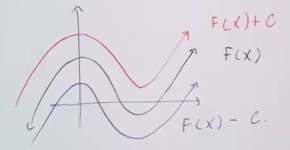
\includegraphics[width=0.4\textwidth]{./Figs/2021-01-11-10-50-53.png}
        % 	\caption{}
        \end{figure}
        \begin{itemize}
            \item No sólo se encuentra $F(x)$ sino también el calor de $C$.
        \end{itemize}
\end{itemize}

\subsection{2 tipos de soluciones para una ED}
\begin{itemize}
    \item La solución general: la solución contiene constantes arbitrarias $c_1,c_2,...,c_n$. (infinitas soluciones)
    \item La solución particular: la solución no contiene constantes arbitrarias. (solución unica)
\end{itemize}

\subsection{Ejemplo}
\begin{enumerate}
    \item $\displaystyle \frac{d y}{d t} + 20y=24$ 
        \begin{center}
           \begin{align*}
               y(t) = \frac{6}{5}+\frac{6}{5}e^{-20t} \\ 
               \text{ Solución particular de la ED. } \\ 
           \end{align*}
        \end{center}
    
    \item $\displaystyle \frac{d ^2y}{d t^2}+4y=0 $ 
        \begin{center}
           \begin{align*}
               y(t) = c_1\cos\p{ 2t } +c_2\sin\p{ 2t } \\ 
               \text{ Solución general. } \\ 
           \end{align*}
        \end{center}
\end{enumerate}

\subsection{Hay una correlación directa entre el orden de la ED y el número de constantes arbitrarias que resultan de la integración}
\begin{itemize}
    \item En general la solución general de una ED depende del orden de la ecuación diferencial.
    \item ED 1er orden: 1 constante arbitraria.
    \item ED 2do orden: 2 constantes arbitraria.
    \item ED n-ésimo orden: n constantes arbitrarias.
\end{itemize}

\subsection{Resolver el siguiente ejercicio}
\begin{itemize}
    \item $\displaystyle \frac{d y}{d t} +20y=24$ 
        \begin{center}
           \begin{align*}
               \frac{d y}{d t} = 24 - 20y \\ 
               \underbrace{\int_{}^{} \frac{dy}{24-20y} = \int_{}^{}dt}_{\text{ Recordar: } \int_{}^{}\frac{d y}{y + b} } = \ln|y+b|+C   \\ 
               -\frac{1}{20}\ln\p{ 24-20y } = t + C \qimplies \text{ ya no hay derivadas entre y } \\
               24-20y = e^{-20t-20C} \\ 
               -20y = -24 - e^{-20t-20C} \\ 
               y = \frac{6}{5}+\frac{1}{20}e^{-20t-20C} \\  
               \text{ Tenemos una solución general, nos deben dar una condición inicial para sacar la solución particular. } \\ 
           \end{align*}
        \end{center}
\end{itemize}
